\documentclass[11pt]{book}
\usepackage{gvv-book}
\usepackage{gvv}
\usepackage[sectionbib,authoryear]{natbib}
\setcounter{secnumdepth}{3}
\setcounter{tocdepth}{2}
\makeindex

\begin{document}
\frontmatter
\tableofcontents
\setcounter{page}{1}
\mainmatter
\chapter{Triangle}
Consider a triangle with vertices
\begin{align}
\label{eq:tri-pts}
\vec{A}=\myvec{1 \\ 3},\,
\vec{B}=\myvec{-3\\0},\,
	\vec{c}=\myvec{0\\4},\,
\end{align}

\section{Vectors}
\section{Median}
\section{Altitude}
\section{Perpendicular Bisector}

\begin{enumerate}[label=\thesection.\arabic*.,ref=\thesection.\theenumi]
\numberwithin{equation}{enumi}

%Question 1.4.1:
\item The equation of the perpendicular bisector of $BC$ is
\begin{align}
\label{eq:tri-perp-bisect}
\brak{\vec{x}-\frac{\vec{B}+\vec{C}}{2}}\brak{\vec{B}-\vec{C}} = 0
\end{align}
Substitute numerical values and find the equations of the perpendicular bisectors of $AB, BC$ and $CA$.
\\	\solution
\begin{enumerate}
    \item $\vec{BC}$: given equation for the perpendicular bisector of $\vec{BC}$:
\begin{align}
    \brak{\vec{x}-\frac{\vec{B}+\vec{C}}{2}}\brak{\vec{B}-\vec{C}} = 0
\end{align}
On substituting the values,
\begin{align}
    \vec{\frac{\vec{B}+\vec{C}}{2}} &= \myvec{\frac{-3}{2} \\ 2} \\
\vec{B}-\vec{C} &= \myvec{-3 \\ -4} \\
\end{align}
solving using matrix multiplication
\begin{align}
\brak{\vec{B}-\vec{C}}^{\top}\brak{\frac{\vec{B}+\vec{C}}{2}}&=0 \\
\brak{\vec{B}-\vec{C}}^{\top} &= \myvec{-3 & -4} \\
\brak{\vec{B}-\vec{C}}^{\top}\brak{\frac{\vec{B}+\vec{C}}{2}}&=\myvec{-3 & -4}\myvec{\frac{-3}{2} \\ 2}\\
&= \frac{-7}{2}
\end{align}
Therefore perpendicular bisector of $\vec{BC}$ is
\begin{align}
    \myvec{-3 & -4}\vec{x}&= \frac{-7}{2}
\end{align}

  \item $\vec{AB}$: similarly the equation for the perpendicular bisector of $\vec{AB}$:
\begin{align}
    \brak{\vec{x}-\frac{\vec{A}+\vec{B}}{2}}\brak{\vec{A}-\vec{B}} = 0
\end{align}
On substituting the values,
\begin{align}
    \vec{\frac{\vec{A}+\vec{B}}{2}} &= \myvec{-1 \\ \frac{3}{2}} \\
\vec{A}-\vec{B} &= \myvec{4 \\ 3} \\
\end{align}
solving using matrix multiplication
\begin{align}
\brak{\vec{A}-\vec{B}}^{\top}\brak{\frac{\vec{A}+\vec{B}}{2}}&=0 \\
\brak{\vec{A}-\vec{B}}^{\top} &= \myvec{4 & 3} \\
\brak{\vec{A}-\vec{B}}^{\top}\brak{\frac{\vec{A}+\vec{B}}{2}}&=\myvec{4 & 3}\myvec{-1 \\ \frac{3}{2}}\\
&= \frac{1}{2}
\end{align}
Therefore perpendicular bisector of $\vec{AB}$ is
\begin{align}
    \myvec{4 & 3}\vec{x}&= \frac{1}{2}
\end{align}

  \item $\vec{CA}$: similarly the equation for the perpendicular bisector of $\vec{CA}$:
\begin{align}
    \brak{\vec{x}-\frac{\vec{C}+\vec{A}}{2}}\brak{\vec{C}-\vec{A}} = 0
\end{align}
On substituting the values,
\begin{align}
    \vec{\frac{\vec{C}+\vec{A}}{2}} &= \myvec{\frac{1}{2} \\ \frac{7}{2}} \\
\vec{C}-\vec{A} &= \myvec{-1 \\ 1} \\
\end{align}
solving using matrix multiplication
\begin{align}
\brak{\vec{C}-\vec{A}}^{\top}\brak{\frac{\vec{C}+\vec{A}}{2}}&=0 \\
\brak{\vec{C}-\vec{A}}^{\top} &= \myvec{-1 & 1} \\
\brak{\vec{C}-\vec{A}}^{\top}\brak{\frac{\vec{C}+\vec{A}}{2}}&=\myvec{-1 & 1}\myvec{\frac{1}{2} \\ \frac{7}{2}}\\
&= 3
\end{align}
Therefore perpendicular bisector of $\vec{BC}$ is
\begin{align}
    \myvec{-1 & 1}\vec{x}&= 3
\end{align}
\end{enumerate}

\begin{figure}[H]
\centering
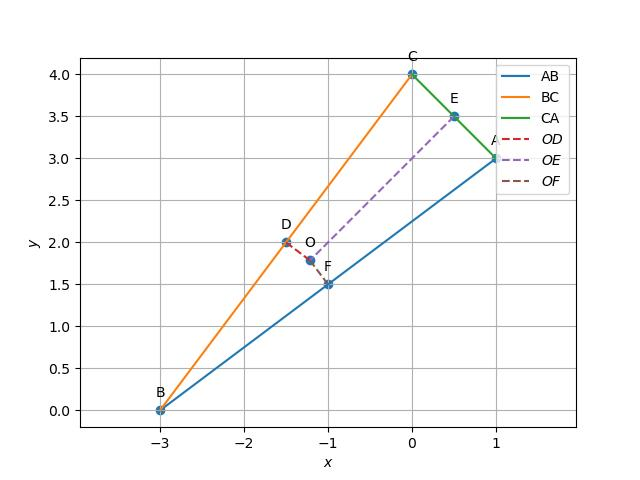
\includegraphics[width=\columnwidth]{/sdcard/hima/geometry/figs/abcdefo.jpg}
\caption{Plot of the perpendicular bisectors}
\label{fig:figure1}
\end{figure}


%Question 1.4.2:
\item Find the intersection $\vec{O}$ of the perpendicular bisectors of $AB$ and $AC$.
 \\
\solution \\
\begin{figure}[H]
\centering
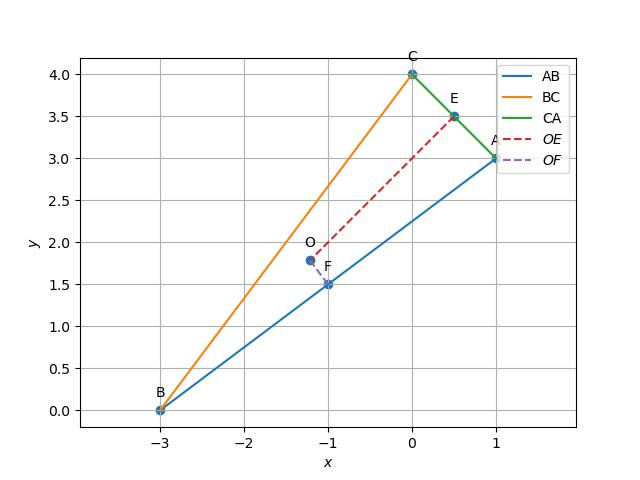
\includegraphics[width=\columnwidth]{/sdcard/hima/geometry/figs/abcefo.jpg}
\caption{$\vec{O}-\vec{E}$ and $\vec{O}-\vec{F}$ are perpendicular bisectors of $\vec{A}-\vec{C}$ and $\vec{A}-\vec{B}$ respectively}
\label{fig:Figure_2}
\end{figure}

Given,
\begin{align}
\vec{A}=\myvec{1 \\ 3},\,
\vec{B}=\myvec{-3\\0},\,
	\vec{c}=\myvec{0\\4},\,
\end{align}

Vector equation of perpendicular bisector of $\vec{A}-\vec{B}$ is
\begin{align}
 (\vec{A}-\vec{B})^\top  \brak{ \vec{x} - \frac{\vec{A}+\vec{B}}{2}} = 0
\end{align}
where,
\begin{align}
\vec{A}+\vec{B}&=\myvec{1\\3}+\myvec{-3\\0}\\
&=\myvec{-2\\3}\\
\vec{A}-\vec{B} &= \myvec{1\\3}-\myvec{-3\\0}\\
&=\myvec{4\\3}\\
\implies (\vec{A}-\vec{B})^\top &= \myvec{4&3}
\end{align}
$\therefore $ The vector equation of $\vec{O}-\vec{F}$ is
\begin{align}
\myvec{4&3} \brak{ \vec{x}-\myvec{-1\\\frac{3}{2}} }&=0\\
\implies \myvec{4&3}\vec{x}&=\myvec{4&3}\myvec{-1\\\frac{3}{2}}
\end{align}
Performing matrix multiplication yields
\begin{align}
\myvec{4&3}\vec{x}&=\frac{1}{2}
\end{align}\\
Vector equation of perpendicular bisector of $\vec{A}-\vec{C}$ is
\begin{align}
(\vec{A}-\vec{C})^\top\brak{ \vec{x} - \frac{\vec{A}+\vec{C}}{2}} = 0
\end{align}
where,
\begin{align}
\vec{A}+\vec{C}&=\myvec{1\\3}+\myvec{0\\4}\\
&=\myvec{1\\7}\\
\vec{A}-\vec{C} &= \myvec{1\\3}-\myvec{0\\4}\\
&=\myvec{1\\-1}\\
\implies (\vec{A}-\vec{C})^\top &= \myvec{1&-1}
\end{align}
$\therefore $ The vector equation of $\vec{O}-\vec{E}$ is
\begin{align}
\myvec{1&-1}\brak{ \vec{x}-\frac{1}{2}\myvec{1\\7}}&=0\\
\implies \myvec{1&-1}\vec{x}&=\frac{1}{2}\myvec{1&-1}\myvec{1\\7}
\end{align}
Performing matrix multiplication yields
\begin{align}
\myvec{1&-1}\vec{x}&=-3
\end{align}

Thus,
\begin{align}
    \myvec{4&3&\frac{3}{2}\\1&-1&\frac{9}{2}} &\xleftrightarrow[]{R_1 \leftarrow \frac{-1}{6} R_1} \myvec{\frac{-2}{3}&\frac{-1}{2}&-1\\1&-1&-3}\\
\myvec{\frac{-2}{3}&\frac{-1}{2}&-1\\1&-1&-3} &\xleftrightarrow[]{R_2\leftarrow R_2 - R_1}
\myvec{\frac{-2}{3}&\frac{-1}{2}& -1\\\frac{-5}{2}&\frac{1}{4}&1}\\
    \myvec{\frac{-2}{3}&\frac{-1}{2}& -1\\\frac{-5}{2}&\frac{1}{4}&1} &\xleftrightarrow[]{R_2 \leftarrow \frac{-1}{2}R_2} \myvec{\frac{-2}{3}&\frac{-1}{2}&-1 \\\frac{-5}{4}&\frac{1}{4}&1}\\
\therefore \myvec{\frac{-2}{3}&\frac{-1}{2}\\\frac{-5}{4}&\frac{1}{4}}\vec{x} &= \myvec{-1\\1}\\
\implies \vec{x}&=\myvec{\frac{5}{4}\\\frac{-5}{4}}
\end{align}
Therefore, the point of intersection of perpendicular bisectors of $\vec{A}-\vec{B}$ and $\vec{A}-\vec{C}$ is $\vec{O} = \myvec{\frac{5}{4}\\ \frac{-5}{4}}$

 %Question 1.4.3:
\item Verify that $\vec{O}$ satisfies
			\eqref{eq:tri-perp-bisect}.
$\vec{O}$ is known as the circumcentre.\\
 \solution
 From the previous question we get,
 \begin{align}
\vec{O}&=\myvec{\frac{5}{4}\\ \frac{-5}{4}} \\
\brak{\vec{x}-\frac{\vec{B}+\vec{C}}{2}}\brak{\vec{B}-\vec{C}} &= 0
\end{align}
when substituted in the above equation,
\begin{align}
	&=\brak{\vec{O}-\frac{\vec{B}+\vec{C}}{2}}.\brak{\vec{B}-\vec{C}}\\
	&=\brak{\myvec{\frac{5}{4}\\ \frac{-5}{4}}- \frac{1}{2}\myvec{-3\\4}}^{\top} \myvec{-3\\-4}\\
	&=\myvec{\frac{-1}{4}& \frac{3}{4}}\myvec{-3\\-4}\\
	&=\frac{-9}{4}
\end{align}
It is hence proved that $\vec{O}$ satisfies the equation \eqref{eq:tri-perp-bisect}
\begin{figure}[H]
\centering
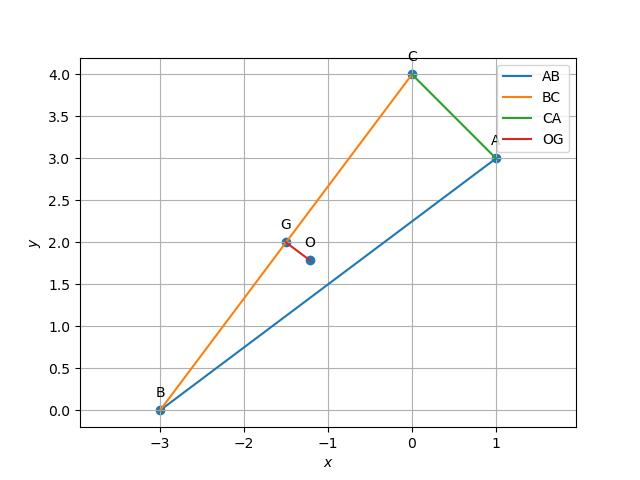
\includegraphics[width=\columnwidth]{/sdcard/hima/geometry/figs/abcog.jpg}
\caption{Circumcenter plotted using python}
\label{fig:Circumcenter to BC}
\end{figure}

 %Question 1.4.4:  
\item Verify that 
\begin{align}
OA = OB = OC 
\end{align} 
\solution
Given \begin{align}
\vec{A} &= \myvec{1\\3}\\
\vec{B} &= \myvec{-3\\0}\\
\vec{C} &= \myvec{0\\4}
\end{align}
From problem-1.4.2 :
\begin{align}
O &= \myvec{\frac{-5}{4} \\ \frac{5}{4}}\\
 &= \myvec{-1.25\\ 1.25}
\end{align}
\begin{enumerate}
\item 
\begin{align}
OA &= \sqrt{(\vec{O}-\vec{A})^{\top}(\vec{O}-\vec{A})}\\
&= \sqrt{\myvec{\frac{1}{4} & \frac{-17}{4}} \myvec{\frac{1}{4}\\ \frac{-17}{4}}}\\
 &= \sqrt{\frac{145}{4}}\\
 &= \frac{\sqrt{145}}{2}
\end{align}
\item 
\begin{align}
OB &= \sqrt{(\vec{O}-\vec{B})^{\top}(\vec{O}-\vec{B})}\\
 &= \sqrt{\myvec{\frac{17}{4} & \frac{-5}{4}} \myvec{\frac{17}{4}\\ \frac{-5}{4}}}\\
 &= \sqrt{\frac{314}{4}}\\
 &= \frac{\sqrt{314}}{2}
\end{align}
\item 
\begin{align}
OC &= \sqrt{(\vec{O}-\vec{C})^{\top}(\vec{O}-\vec{C})}\\
 &= \sqrt{\myvec{\frac{5}{4} & \frac{-21}{4}}  \myvec{\frac{5}{4}\\ \frac{-21}{4}}}\\
 &= \sqrt{\frac{466}{4}}\\
 &= \sqrt{\frac{233}{2}}\\
\end{align}
\end{enumerate}
From above, 
\begin{align}
OA = OB = OC
\end{align}
Hence verified.

%Question 1.4.5:
\item Draw the circle with centre at $\vec{O}$ and radius 
\begin{align}
R = OA
\end{align}
This is known as the {\em circumradius}. \\
\solution
Given
\begin{align}
\vec{A} &= \myvec{1\\3}\\
\vec{B} &= \myvec{-3\\0}\\
\vec{C} &= \myvec{0\\4}
\end{align}
From Q1.4.2, the circumcentre is
\begin{align}
\vec{O} = \myvec{\frac{5}{4}\\ \frac{-5}{4}}
\end{align}
Now we will calculate the radius,
\begin{align}
      R &= OA\\
        &= \norm{\vec{A} - \vec{O}}\\
        &= \norm{\myvec{1\\3} - \myvec{\frac{5}{4}\\ \frac{-5}{4}}}\\
        &= \norm{\myvec{\frac{1}{4}\\ \frac{-17}{4}}}\\
        &=\sqrt{\myvec{\frac{1}{4} & \frac{-17}{4}}\myvec{\frac{1}{4} \\ \frac{-17}{4}}} \\
        &= \frac{\sqrt{145}}{2}
\end{align}
see \figref{fig:circumcircle with centre O}
\begin{figure}[H]
\centering
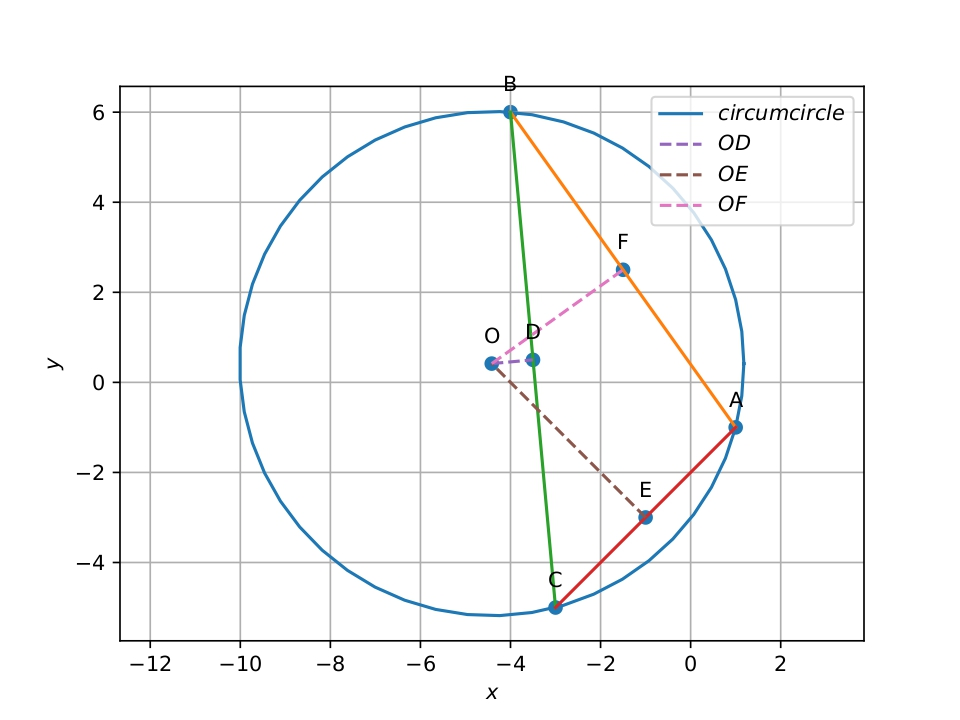
\includegraphics[width=\columnwidth]{/sdcard/hima/geometry/figs/circumcircle.jpg}
\caption{circumcircle of Triangle ABC with centre O}
\label{fig:circumcircle with centre O}	
\end{figure}

 %Question 1.4.6:
\item Verify that 
\begin{align}
\angle BOC = 2\angle BAC.
\end{align}\\
 \solution
\begin{enumerate}
\item To find  the value of $\angle{BOC}$ :
\begin{align}
\vec{B}-\vec{O}
          &=\myvec{\frac{-17}{4}\\\frac{5}{4}} \\
\vec{C}-\vec{O}
         & =\myvec{-\frac{-5}{4}\\\frac{21}{4}}
	  \\
\implies \brak{\vec{B}-\vec{O}}^{\top}\brak{\vec{C}-\vec{O}}&=\frac{5}{4}\\
	\implies \norm{\vec{B}-\vec{O}}&=  \sqrt{\frac{157}{8}} \\
	\norm{\vec{C}-\vec{O}} &=  \sqrt{\frac{233}{8}}
\end{align}
Thus,
\begin{align}
\cos{BOC}&=\frac{\brak{\vec{B}-\vec{O}}^{\top}\brak{\vec{C}-\vec{O}}}{\norm{\vec{B}-\vec{O}}\norm{\vec{C}-\vec{O}}}
=\frac{10}{191}\\
\implies\angle{BOC}&=\cos^{-1}\brak{\frac{10}{191}}
\\
	&=1.518\degree
\end{align}
Taking the reflex of above angle we get 
\begin{align}
    \angle{BOC}&=360\degree-1.518\degree \\
    &= 358.482\degree
\end{align}
	\item To find  the value of $\angle{BAC}$ :
\begin{align}
\vec{B}-\vec{A}&=\myvec{-4\\-3} \\
\vec{C}-\vec{A}&=\myvec{-1\\1}
\\
\implies \brak{\vec{B}-\vec{A}}^{\top}\brak{\vec{C}-\vec{A}}&=-6
\\
	\norm{\vec{B}-\vec{A}}&= \sqrt{25}= 5
	\norm{\vec{C}-\vec{A}}= \sqrt{2}
\end{align}
Thus,
\begin{align}
\cos{BAC}&=\frac{\brak{\vec{B}-\vec{A}}^{\top}\brak{\vec{C}-\vec{A}}}{\norm{\vec{B}-\vec{A}}\norm{\vec{C}-\vec{A}}}
=\frac{1}{5\sqrt{2}}\\
\implies\angle{BAC}&=\cos^{-1}\brak{\frac{1}{5\sqrt{2}}}\\
&=1.4288\degree \label{eq:2}  \\
2\times\angle{BAC} &= 2.8576
\end{align}
From \eqref{eq:2} and \eqref{eq:1},
\begin{align}
2\times\angle{BAC}
= \angle{BOC}
\end{align}
Hence Verified
\end{enumerate}

  %Question 1.4.7:
\item Let 
\begin{align}
\vec{P} = \myvec{\cos \theta & -\sin \theta \\ \sin \theta & \cos \theta}
\end{align}
Find $\theta$ if 
\begin{align}
\vec{C}-\vec{O}=\vec{P}\brak{\vec{A}-\vec{O}}
\end{align}
\solution
\begin{align}
    \vec{C}-\vec{O}
          & =\myvec{\frac{-5}{4}\\\frac{21}{4}}\\
\vec{A}-\vec{O}
         & =\myvec{\frac{-1}{4}\\\frac{17}{4}}
	  \\
\vec{P} &= \myvec{\cos \theta & -\sin \theta \\ \sin \theta & \cos \theta} \\
   \vec{C}-\vec{O}&=\vec{P}\brak{\vec{A}-\vec{O}} \label{eq:1.4.7.6}
\end{align}
 Now from \eqref{eq:1.4.7.6}
 \begin{align}
 \myvec{\frac{-5}{4}\\\frac{21}{4}}&= \myvec{\cos \theta & -\sin \theta \\ \sin \theta & \cos \theta} \myvec{\frac{-1}{4}\\\frac{17}{4}}    
 \end{align}
solving using matrix multiplication,we get
\begin{align}
    \myvec{\frac{-5}{4}\\\frac{21}{4}}&=\myvec{ \frac{1}{4}\cos\theta + \frac{17}{4}\sin\theta \\ \frac{-1}{4}\sin\theta + \frac{17}{4}\cos\theta}
\end{align}
Comparing on Both sides ,we get
\begin{align}
     \frac{1}{4}\cos\theta + \frac{17}{4}\sin\theta &= \frac{-5}{4}  \label{eq:1.4.7.9}\\
 \frac{1}{4}\sin\theta + \frac{17}{4}\cos\theta &= \frac{21}{4} \label{eq:1.4.7.10}
\end{align}
On solving equations \eqref{eq:1.4.7.9}  and \eqref{eq:1.4.7.10}
\begin{align}
    \cos\theta&= \frac{2900}{901} \\
    \sin\theta&= \frac{-53}{145} \\
    \theta &=\cos^{-1}\frac{2900}{901} \\
            &= 0.99 \\
            \therefore \theta = 0.99
\end{align}
\end{enumerate}
\end{document}
